%\documentclass{article}
\documentclass[aps,reprint,amsmath,amssymb]{revtex4-2}


%\usepackage{arxiv}

\usepackage[utf8]{inputenc} % allow utf-8 input
\usepackage[T1]{fontenc}    % use 8-bit T1 fonts
\usepackage{hyperref}       % hyperlinks
\hypersetup{colorlinks=true,urlcolor=red}
\usepackage{url}            % simple URL typesetting
\usepackage{booktabs}       % professional-quality tables
\usepackage{amsfonts}       % blackboard math symbols
\usepackage{nicefrac}       % compact symbols for 1/2, etc.
\usepackage{microtype}      % microtypography
\usepackage{lipsum}
\usepackage{graphicx}
\graphicspath{ {./images/} }
%\usepackage[numbers,sort&compress]{natbib}
\usepackage{siunitx}

\begin{document}

\title{Adatoms in the surface Ullmann coupling}

\author{Zhenzhe Zhang}
\author{Dmitrii F. Perepichka}
\email{dmitrii.perepichka@mcgill.ca}
\author{Rustam Z. Khaliullin}
\email{rustam.khaliullin@mcgill.ca}
\affiliation{Department of Chemistry, McGill University, 801 Sherbrooke St. West, Montreal, QC H3A 0B8, Canada}

\begin{abstract}
This manuscript reviews the results of experimental and computational studies of the surface Ullmann coupling that shed light on the role of surface adatoms in its mechanism. A particular focus is on the early stages of the polymerization and coupling of two monomers.
\end{abstract}

\maketitle



\section{Introduction}

\subsection{Ullmann coupling in solution}

\begin{figure}[b]
\centering
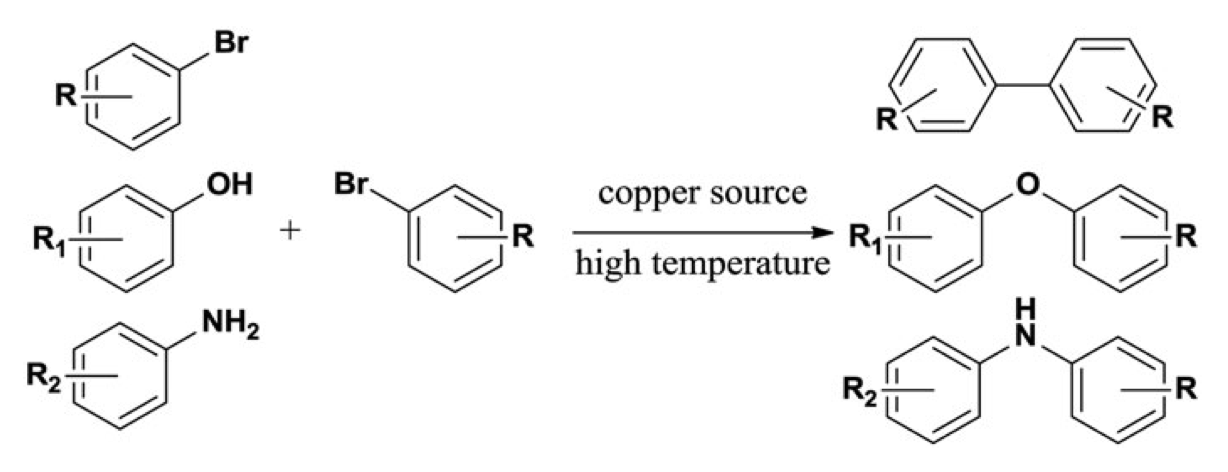
\includegraphics[width=0.98\columnwidth]{Fig/classical.png}
%RZZK: "Cu source" -> "Cu source"; "high T" -> "high T"(ZZ: solved)
\caption{Ullmann coupling reaction}
\label{fig:initial}
\end{figure}

%ZZ:(Cu is catalyst?)
%ZZ:(only refer to C-C bond)
In 1901, Fritz Ullmann discovered~\cite{ullmann_01} a coupling reaction between two aryl halides that results in the creation of a C--C bond between the aromatic rings 
in the presence of the equivalent amount of Cu powder.
%RZK is the previous statement correct? or should we use the alternative ending below?: in the presence of Cu-containing catalysts.
%ZZ:(figure 2 did not show Cu is a catalysis) Our Figure 2?
Today, terms ``classical'' Ullmann, Ullmann-type or simply Ullmann reaction refers to a family of Cu-catalyzed nucleophilic aromatic substitution reactions between aryl halides and various (RZK: aromatic?) nucleophiles that lead to the formation of C--C and C--heteroatom bonds 
%
%RZZK-original: The ``classical'' Ullmann reaction, named after Fritz Ullmann who discovered it in 1901~\cite{ullmann_01}, is a coupling reaction between two aryl halides that results in the creation of a C--C bond between the aromatic rings in the presence of Cu-containing catalysts (figure.~\ref{fig:classical}).
%
%ZHZ-new: Cu-catalyzed arylation mainly referred to the formation of C--C and C--heteroatom bonds have acquired great importance in the last decades. This type of reaction can trace back to one of the oldest reactions, name Ullmann reactions (figure.~\ref{fig:initial}). With increasing understanding of the mechanism of transition-metal mediated reactions, the scope of the Ullmann coupling reaction has been extended to new reactants and catalysts.
%
such as C--N~\cite{ullmann_02, ullmann_03}, C--O~\cite{ullmann_04}, C--S~\cite{ullmann_05} and C--P~\cite{ullmann_21,ullmann_22} bonds (F
Figure.~\ref{fig:classical}). 
%
%RZK: diary ether??? phosphines and/or phosphites?
Depending on the type of a bond created, reactants in the Ullmann coupling reaction include aromatic amines~\cite{ullmann_17,ullmann_18} and amides~\cite{ullmann_19,ullmann_20} for the C--N bond creation; phosphines(PH3)~\cite{ullmann_21,ullmann_22} to achieve the arylation of phosphites(HPO3[2-]); carboxylic acids~\cite{ullmann_23}, diaryl ether~\cite{ullmann_24}, phenols~\cite{ullmann_25} and other oxygen-containing species~\cite{ullmann_26,ullmann_27,ullmann_28} to obtain C--O bond products.
%
While iodine and bromine serve as leaving groups most often, the usage of the tosylate leaving group has also been reported in the Ullmann coupling~\cite{ullmann_15}. 
%
In addition to Cu(0), different Cu(I) and Cu(II) salts and oxides -- including CuI~\cite{ullmann_07,ullmann_08,ullmann_09}, CuBr~\cite{ullmann_10,ullmann_11}, CuCl~\cite{ullmann_13}, Cu$_2$O~\cite{ullmann_12}, Cu(acca)$_2$~\cite{ullmann_14}, Cu(OTf)$_2$~\cite{ullmann_15}, CuO~\cite{ullmann_16} -- have been used as catalysts in the Ullmann reaction.
% RZZK: other metals as catalysts? Yes. But is it called Ullmann in this case? 

\begin{figure}[thb]
\centering
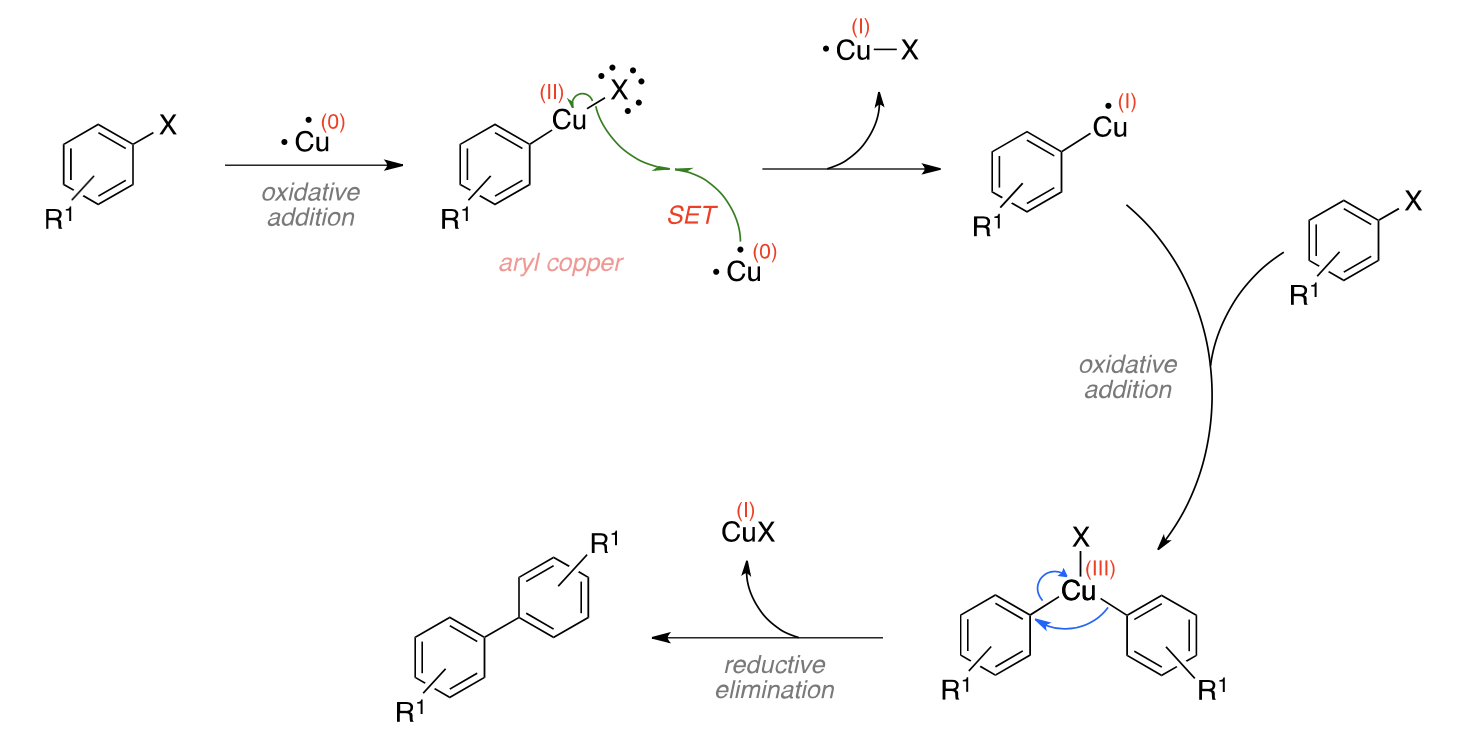
\includegraphics[width=0.98\columnwidth]{Fig/classical-mechanism.png}
% RZZK: This looks like a very clear figure that explains the mechanism. Some modifications will be necessary LATER: 
% * convert into a one-line page-wide scheme. 
% * clarify whether Cu is a reactant or catalyst. If latter, it is unclear how Cu returns to its initial Cu(0) form.
% * why Cu(0) is shown with two electrons? Is it better to show Cu without its electrons?
% * define SET: single-electron transfer?
% * How is it possible to use Cu(II) salts as catalysts/reagents?
\caption{Mechanism of the Ullmann coupling reaction.}
\label{fig:classical}
\end{figure}

%RZZK, our next major task is to describe the mechanism using the commonly accepted terminology. 
It is widely accepted that the Ullmann coupling proceeds via the formation of an organometallic intermediate (Figure.~\ref{fig:classical}). 
This intermediate then reacts with another precursor with the formation of a ZZZ and a subsequent reductive elimination to form biaryl moieties (Figure.~\ref{fig:classical}). 

Cu-catalyzed coupling has acquired great significance in the last decade due to its advantages such as (1) Cu is a cheaper alternative to palladium, platinum or rhodium; (2) avoidance of the halogen side-product; and (3) air or oxygen can act as oxidant. However, drawbacks still exit for large-scale development: (1) harsh conditions are necessary like high T and polar solvents with high boiling point; (2) poor solubility of many Cu compounds in solvent; (3) poor functional group tolerance. %RZZK: Despite a variety of limitations ranging from harsh reaction conditions~\cite{RZZK} and erratic yields~\cite{RZZK}, the Ullmann coupling has become and still remains one of the key reactions to build C-C bonds in organic synthesis. 

Recent advances in the traditional Ullmann coupling reaction in solution have been reviewed by several authors~\cite{ullmann_29,ullmann_30,ullmann_31,ullmann_32}.

%RZK: Reaction mechanism figure for Cu(I) or Cu(II). Catalyst regeneration.

\subsection{Surface Ullmann coupling}

A recent surge of interest in electronic devices based on low-dimensional organic nanostructures with $\pi$-conjugated backbones has led to a renewed attention to the Ullmann coupling reaction. 
In the case of low-dimensional materials, the well-established ability of the Ullmann coupling to create bonds between aromatic carbon atoms and couple their $\pi$ systems have been transferred from solution to metal surfaces, which serve as both a low-dimensional confining template and catalyst. 
The on-surface Ullmann reaction is currently viewed as a promising bottom-up strategy to assemble, in mild conditions, one- and two-dimensional organic polymers with high degree of control of their electronic properties~\cite{ullmann_33}. 
It is important to note that the term Ullmann coupling has been extended to refer to reactions on metals other than than Cu such as silver and gold. 

% RZZK. They say, phenyl is parallel to the surface. Was it confirmed later?
One of the first fundamental studies of the surface-confined coupling of iodobenzene to biphenyl under ultrahigh vacuum (UHV) condition was reported by Xi \textit{et al.} in 1992~\cite{sur_sci01}.
%
The intermediate species of the same reaction were inspected using STM imaging by Weiss and coworkers in 1998~\cite{langm01}.
% RZZK: I removed the following reference because it cannot be classified as Ullmann coupling
% STM tip was further utilized to achieve a chain polymerization, which result in polydiacetylene from diacetylene compounds in 2000~\cite{ullmann_34}.
%
In 2004, it was demonstrated that linear \emph{protopolymers} -- aligned monomer units of a polymer that have not yet reacted to form the final polymer -- can be obtained by depositing \textit{para}-diiodobenzene on Cu(111) at 77 K~\cite{jacs01}. 
%
Remarkably, the first synthesis of covalently-bonded nanostructures from molecular building blocks on metal surfaces under vacuum has employed the Ullmann reaction: the coupling between brominated tetraphenyl-porphyrins on the Au(111) surface was performed by Grill and coworkers in 2007~\cite{Naturenano2007}.

Since then, surface Ullmann coupling has become one of the most representative on-surface synthesis scheme and has been utilized to create a variety of covalently-linked extended aromatic systems from halogenated aryl precursors on multiple metal surfaces~\cite{ullmann_34}. 
%RZK: more reviews from our list must be cited here


\subsection{Mechanism of surface Ullmann coupling}

Although multiple covalently-bonded nanostructures have been obtained on metal surfaces via Ullmann coupling, our knowledge of the mechanism of the surface processes still remains fragmentary. 
%
A thorough understanding of the mechanism of surface Ullmann coupling reaction will enable rational, faster, more precise design of the halogenated precursors, well-matched to a chosen metal surface.
%
%RZZK: the following sentence does not belong here.
%The organometallic intermediates have been proven in existence in the mechanism investigation. %
%RZK: note how I refer to figures. Do not abbreviate "Fig.", use non-breaking space ~.(ZZ: solved)
The overall coupling process can be divided into elementary steps depicted in Figure.~\ref{fig_mecha} and described in detail below.
%RZZK: After the mechanism of the in-solution process is describe, add a sentence or two on how the in-solvent and on-surface mechanisms are related. Should we opt for a similar electron-based picture of the mechanism for the on-surface process?

\begin{figure*}[htb]
\centering
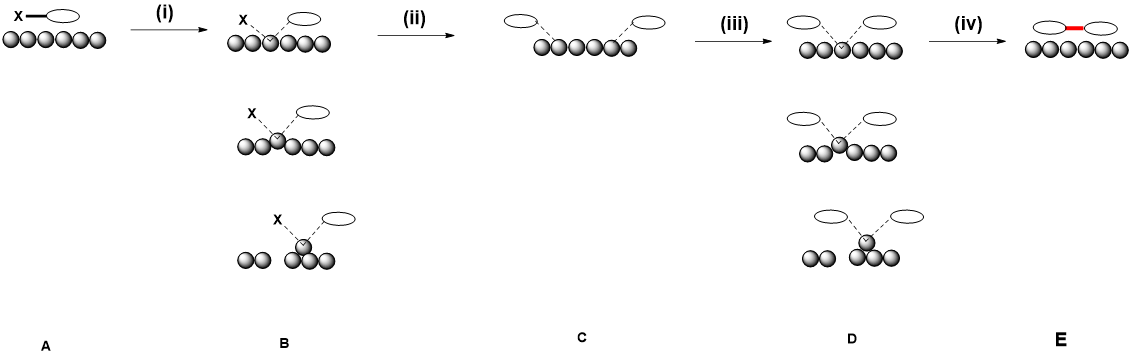
\includegraphics[width=0.98\textwidth]{Fig/mechanism.png}
\caption{Five steps in surface Ullmann coupling}
\label{fig_mecha}
\end{figure*}

%%\begin{enumerate}[align=left, itemindent=2em, label=(\roman*)]
    %%\item Dehalogenation of Precursors [The fundamental step is the %%disassociate of halogens, the cleavage of C-X bonds (X = halogens) is %%usually activated by thermal, electron-induced and photon-simulated. %%The energy will vary from 0.05 ~ 0.80 eV with different X on different %%coinage surfaces.]
    %%\item Diffusion of single Dehalogenlated 'Radicals' [The removal of %%halogens from precursors results in unsaturated carbons (radicals), %%which interact with metal atoms to form C-Metal radical (C = %%dehalogenated precursor and Metal = Au, Ag or Cu). C-Metal radical %%will diffuse on metal surface and the metal atom interacting with the %%radical will shift.]
    %%\item The Formation of Organometallic Intermediates C-Metal-C from Two %%Single Radicals [Diffusion brings two single radical close to each %%other, and then these two species would form a dimerized %%organometallic intermediate before the appearance of coupling product]
    %%\item The Formation of Carbon-Carbon Bond []
    %%\item Diffusion of Coupling Product []
%%\end{enumerate}  


\subsubsection{Dehalogenation}

%RZZK: carbon or heteroatom?
%RZZK: no reference to the figure steps
The first fundamental step of the surface Ullmann coupling is the dissociative dehalogenation of organic precursors adsorbed on the surface. In this step, carbon-halogen bonds are broken while carbon-metal and halogen-metal bonds are formed. The thermodynamics and kinetics of the process primarily determined by the relative strength of the broken and formed bonds. 
Bond strength (X = Halogen, M = Metal): 
%RZZK: I did not check the actual strength for these bonds, please check the trends
%
\begin{eqnarray}
\text{C -- Cl} > \text{C -- Br} > \text{C -- I} \\
\text{Cu -- C} > \text{Ag -- C} > \text{Au -- C} \\
\text{Cu -- X} > \text{Ag -- X} > \text{Au -- X} \\
\text{M -- Cl} > \text{M -- Br} > \text{M -- I}
\end{eqnarray}
%
%RZZK: What of the two factors influence this step more: the nature of the hallogen or the nature of the metal? Is it possible to arrange the nine M--X cases in term of bond strength? It is possible to do a whole study on the predicting the energetics of this step based on bond energies. This can be done in the results and discussion, if necessary.
This data also indicates the distinct influence of surfaces, which has been proven in experiment of bromobenzene and iodobenzene. For instance, the dissociaton of iodobenzene occurs at approximately 175~K on Cu(111)~\cite{sur_sci01}, 200~K on Ag(111)~\cite{sur_sci02} and 250~K on Au (111)~\cite{sur_sci03}. The same trend has been demonstrated by bromobenzene with a higher T on all surfaces.

In 2013, Björk Jonas~\cite{jacs2013} proposed an activation barrier of 0.4-1.0 eV for exothermic dehalogenation by DFT simulations. In specific, bromobenzene and iodobenzene on Au(111), Ag(111) and Cu(111) surface displayed different reactivity, i.e., the activation barrier and reaction energy both decrease in the order Au > Ag > Cu, and for all surfaces studied, iodine substituents are 0.1-0.5 eV lower than bromine ones in dehalogenation (Figure.~\ref{fig:dehalo}). The trend is plausible due to the Bond-dissociation energy(BDE) of C-I is ~0.65 eV lower than C-Br\cite{Arpc1982}.

\begin{figure}[htb]
\centering
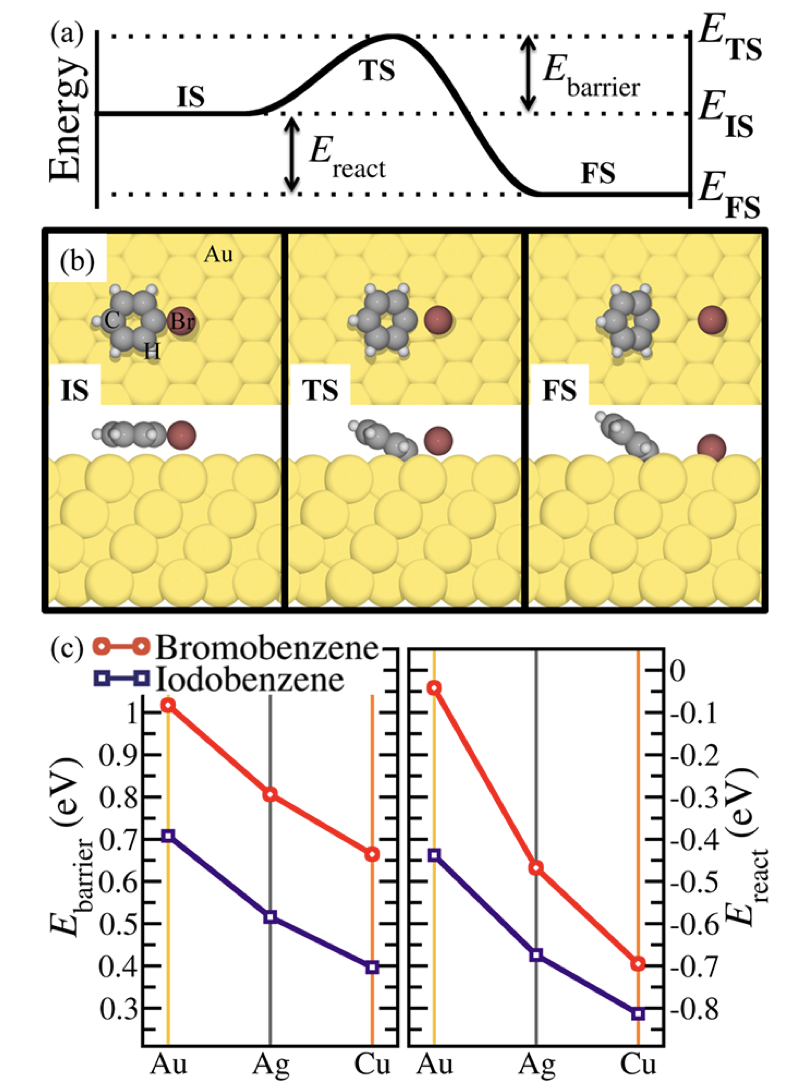
\includegraphics[width=0.98\columnwidth]{Fig/dehalogentaion.png}
\caption{Dehalogenation energy. RZK: Detailed description of the figure. Take a look at the original publication. Reprinted from~\cite{RZK} with permission of American Chemical Society or PUBLISHER. See the LaTeX comment below.}
%%RZK: If you take a figure from a publication it is very important to cite the work and obtain publisher's permission. We need to make sure that all our borrowed figures satisfy copyright permissions. For example, see: https://www.stm-assoc.org/2016_01_05_Guidelines_for_Quotation_From_Journal_Articles.pdf
\label{fig:dehalo}
\end{figure}

%RZZK: diffusion of halogen atoms?
%RZZK: dissociation products?
\subsubsection{Diffusion of organometallic species}

%RZK. Compare the two versions.
%The dehalogenation step produces unsaturated carbons (surface-stabilized single radicals), where the dangling bonds of the unsaturated carbons bind to the adjacent metal atom. The diffusion accessibility of single radicals play a decisive role in further coupling process. 
The dehalogenation step produces organometallic intermediates with carbon atoms covalently bonded directly to surface metal atoms. On the next key step, these intermediates approach each other by diffusion. 
%
% RZK: note that I use phenyl GROUPS, not RADICALS. (ZZ: solved) 
The diffusion process of dehalogenated organic species has been observed experimentally and studied computationally. For example, an STM imaging has revealed that dehalogenated phenyl groups diffuse on Cu(111) at 77~K~\cite{langm01}. The calculated low energy barrier of the diffusion, $\sim$0.09~eV, is consistent with the experimental T~\cite{RZK-same-article?}. Calculations has also shown that phenyl groups, which are tilted at $\sim 36^\circ$ with respect to the surface~\cite{pccp2010}, overturn as shown in Figure.~\ref{fig:4} during the diffusion to bind to a nearby atom. 

%RZK: Are their any trends in the diffusion activation barriers for different metals?

\begin{figure}[htb]
\centering
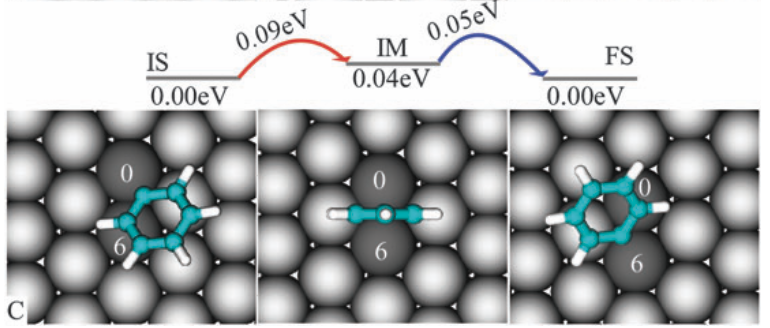
\includegraphics[width=0.98\columnwidth]{Fig/overturn.png}
\caption{overturn} %RZK: better caption, copyright.
\label{fig:4}
\end{figure}

%RZZK do we need to keep the following or is it too obvious?: The diffusion energy barrier and the tilt angle between single radical and substrate will change with the size increasing of reactant molecules.

%RZK: What happens to halogen atoms? How mobile are they? A couple of sentences.


\subsubsection{Formation of dimerized organometallic intermediates}

%RZK: "close" or do they have to be bonded to the same metal atom?
A dimerized organometallic intermediate based on carbon-metal-carbon interlinks forms when two single phenyl groups diffuse close to each other. 
These carbon-metal-carbon bridges have been revealed in many cases. In 2011, Wang Weihua~\cite{jacs2011} studied the organometallic intermediate of surface Ullmann coupling from dibromoterphenyl to polyphenylene by STM and DFT calculations. When the T goes to 300 K, Br atoms are dissociated from the phenyl group. However, there is 4.8 \si{\angstrom} difference in length between the linear periodic structure from STM image and terphenyl group (ph)$_{3}$ by DFT calculation. A Cu atom was proposed to stay in the 4.8 \si{\angstrom} gap and connect two adjacent carbon atoms. And both the performed tunneling spectra (dI/dV) of one periodic unit and the calculated projected density of states (PDOS) of (ph)$_{3}$ and Cu atom show the value at ~2.7 eV, which further proves the C-Cu-C bridges in organometallic intermediate structures. Same method has been used by Chung Kyung-Hoon~\cite{PCCP2012} with the same molecule on Ag(111). C-Ag-C bridges are observed and demonstrated in the organometallic intermediates.

\begin{figure}[ht]
\centering
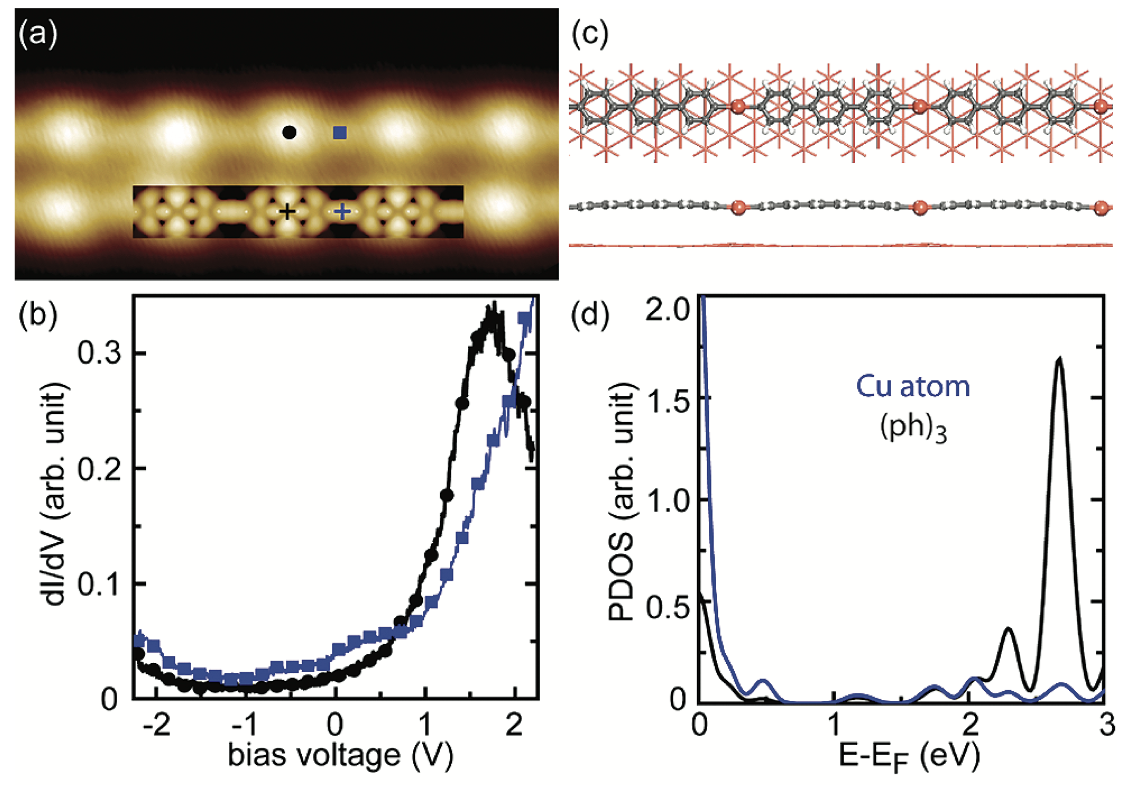
\includegraphics[width=0.98\columnwidth]{Fig/Organometallic.png}
\caption{Carbon-Metal-Carbon Bridges in Organometallic Intermediate}
\label{fig:organ}
\end{figure}


\subsubsection{Formation of the C--C bond}

Upon further annealing on the dimerized organometallic intermediates, the metal atoms are released, while two metalstable bonds are irreversibly converted into covalent bonds. In 2016, Di Giovannantonio~\cite{jacs2016} reported the dimerization and trimerization of 1,4-dibromobenzene on Cu(100). It is found that organometallic intermediate is a relative stable phase in potential energy surface. A 0.7 eV of activation energy is required from the relatively stable organometallic intermediate to dimerized coupling product. And a 0.2 eV of activation is needed from dimerized coupling product the trimer. This result is consistent with the experimental data, which was investigated by Di Giovannantonio~\cite{acsnano2013} in 2013. Same monomer dibromobenzene was deposited on Cu(100) surface, under STM image, organometalic intermediates are formed at RT, while the final coupling product need the T up to 500 K.

\begin{figure*}[ht]
\centering
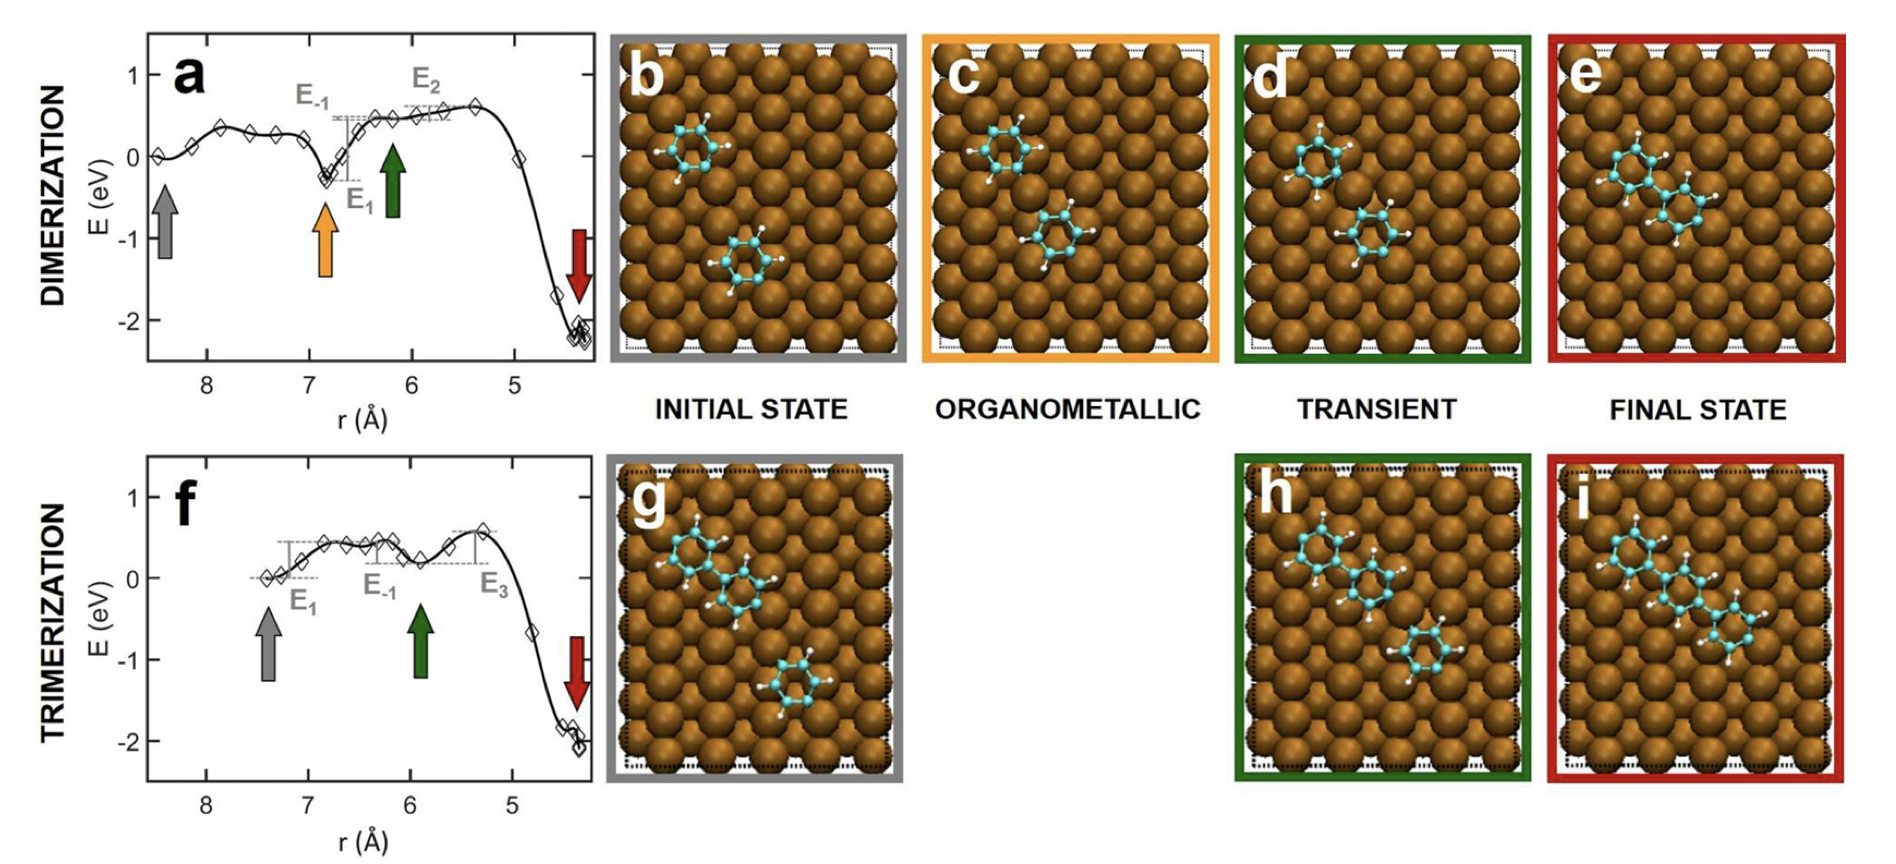
\includegraphics[width=0.98\textwidth]{Fig/Dimer_trimer.png}
\caption{Energy curve for dimerization and trimerizaiton coupling}
\label{fig:dimer}
\end{figure*}


\subsection{Role of adatoms in the surface Ullmann coupling} 

Metal atoms are involved in the mechanism of Ullmann coupling containing five steps mentioned above. Investigation on the role of metal atoms in intermediates delivered a long-existence argument.
%%%%%%%%%%%%%%%%%%%%%%%%%%%%%%%%%%%%%%%%%%%%%%%%%%%%%%%%%%%%%%%%%%%%%%%%%%
%%The metal atoms may come from: (1) adatoms residing on metal surface; %%(2) metal atoms reside inside the metal surface. These two possibilities %%have been explored both experimentally and computationally in first %%three steps. \\
%%%%%%%%%%%%%%%%%%%%%%%%%%%%%%%%%%%%%%%%%%%%%%%%%%%%%%%%%%%%%%%%%%%%%%%%%%
Here the two terminology $Nature$ and $Origin$ will be used to distinguish the metal atoms in Ullmann coupling.
The nature of metal atoms: metal atoms can come from (1)surface atom or (2)adatoms.
The origin of adatoms: adatoms may come from (1)pre-exsiting adatom due to the the thermal fluctuations (At 298 K, the concentration of free adatoms and mono-vacancies $10^{-9}$ on Cu and Ag surfaces It increases to the order of $10^{-5}$ around 500 K). It increases to the order of 10 around 500K)[Figure.~\ref{fig:2D-gas}] or (2)pulled out by the intermediates in Ullmann coupling. The nature of metal atoms and the origin of adatoms have been explored experimentally and computationally.

\begin{figure}[ht]
\centering
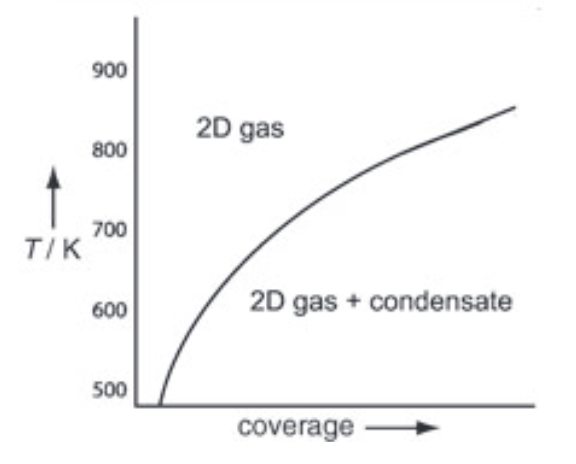
\includegraphics[width=0.98\columnwidth]{Fig/2D-gas.png}
\caption{Adatoms Consentration on Metal at Elevated T}
\label{fig:2D-gas}
\end{figure}


\subsubsection{Dehalogenation of precursors}

Evidences already presented that metal adatoms are in assistance in the process of dehalogenation. In 2017, Barton Dennis~\cite{chemeurope2017} explored the role of adatoms in the dehalogenation with iodobenzene on three different surfaces including Au(111), Ag(111) and Cu(111) based on DFT calculations.They compared the energetics of adatom formation on pristine metal surface and in the presence of iodobenzene. The comparison has shown that the energy of extracting a metal atom from the surface is decreased substantially from the 1.12-1.71~eV range to 0.13-0.24~eV range. Furthermore, the calculations have shown that the energy released in the process of adsorption of idobenzene and formation of metalorganic intermediates is sufficent to compensate the energy required for a metal atom extraction. [Figure.~\ref{fig:3}]

\begin{figure}[ht]
\centering
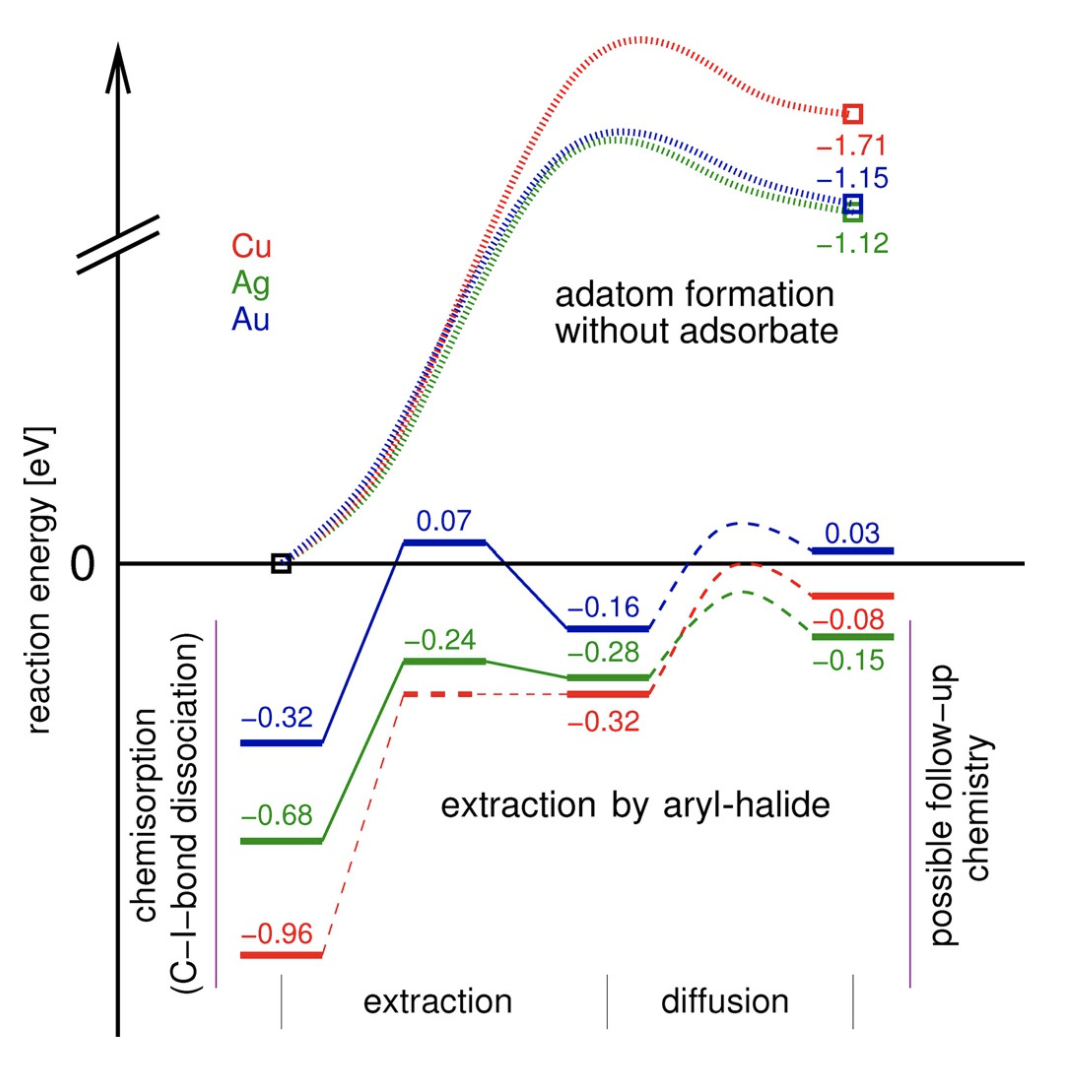
\includegraphics[width=0.98\columnwidth]{Fig/Adatom-formation.png}
\caption{Energetics of adatoms formation}
\label{fig:3}
\end{figure}


\subsubsection{Diffusion of two dehalogenlated phenyl groups}

The diffusion process is involved in the interaction between single precursor group and metal atom. 
In 2018, Nagoya Akihiro~\cite{jpcc2018} investigated the mechanism of Ullmann coupling of 7,10-dibromofluoranthene (Br$_{2}$FL) on Au(111) via DFT calculations. Compared to simple phenyl rings that tend to form ~$36^\circ$ tilt angle with Cu(111) surface~\cite{pccp2010}, the monobromo FL with only one Br atom removed stays almost parallel to Au(111) surface due to steric repulsion from the large backbone of BrFL group and the substrate. And BrFL group is found to lift surface Au atom out by 1.9 \si{\angstrom} from its initial position, which is much larger than 0.16 \si{\angstrom} produced by a phenyl ring. 

Ebeling Danie~\cite{acsnano2019} also indicated 4-bromo-3$^{''}$-iodo-$p$-terphenyl group interacts with the Cu atom inside the surface, and partially lift the Cu atom out from the surface while diffuses on Cu(111) surface. The conclusion 

\begin{figure}[ht]
\centering
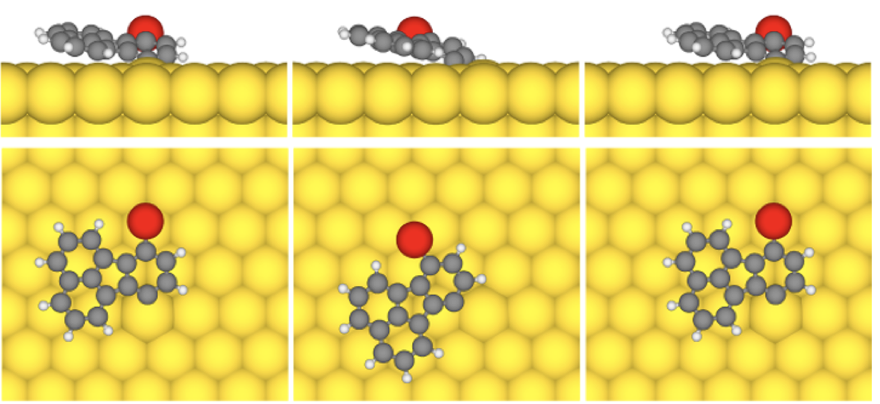
\includegraphics[width=0.98\columnwidth]{Fig/Diffusion_path.png}
\caption{Diffusion}
\label{fig:diff}
\end{figure}


\subsubsection{Formation of organometallic intermediates from two precursor groups}

The nature of the metal atom in dimerized organometallic intermediate has also been investigated through various approaches. In 2017, Zint Sören~\cite{acsnano2017} analyzed structures of intermediates in the polymerization of bromotriphenylene to bistriphenylene on Cu(111) surface using STM/AFM and DFT calculations. Two computational models were considered: two triphenylene molecules bonded to an fully-out-of-surface adatom and two precursors bonded to an atom partially lifted from Cu surface [Figure.~\ref{fig:5}]. It has been concluded that the structures observed in AFM are more consistent with computational adatom models. In particular, the C...C distance in organometallic intermediate is of 3.9 \si{\angstrom} measured by AFM, which is closer to the Cu adatom model (3.86 \si{\angstrom}) compared to the partially-lifted Cu atom model (3.42 \si{\angstrom}). Furthermore, the energy of formation of the adatom-containing intermediate from distant precursors is 1.74~eV lower than that of the intermediate with a partially lifted atoms. 


\begin{figure}[ht]
\centering
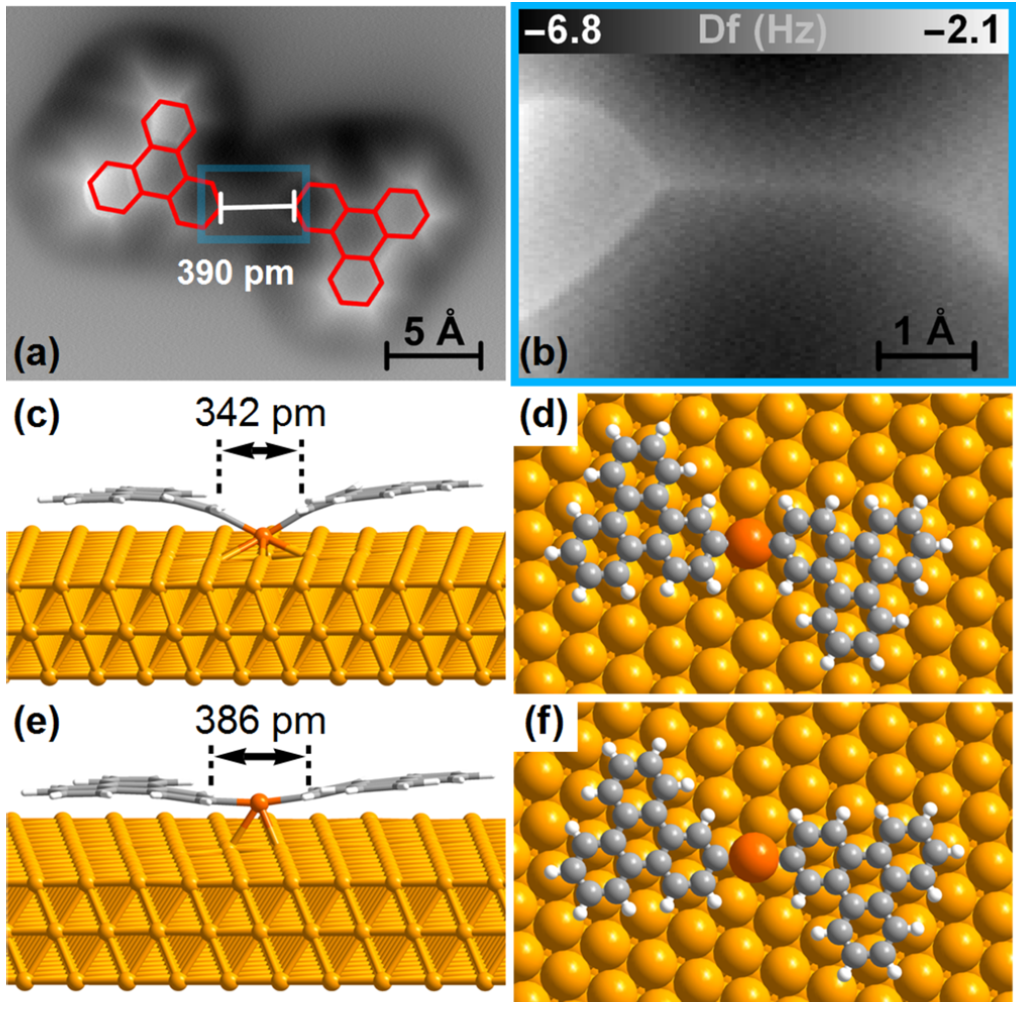
\includegraphics[width=0.98\columnwidth]{Fig/distance.png}
\caption{distance}
\label{fig:5}
\end{figure}

%%ZHZH Dima suggests partial lifting should be discussed separately.

Then in 2019, not only the nature of metal atoms, but also the origin of the adatoms was discussed. The 2019 study of 4‐Bromo-3′′- iodo‐p‐terphenyl coupling on Cu(111), comparing experimentally and simulated AFM image, the Cu atoms in dimerized organometallic intermediate was again proven to be adatoms~\cite{acsnano2019}. It was further suggested that these adatoms are generated by the extraction of two close single precursor groups, instead of pre-exsiting adatoms from a statistic study of all intermediates species in the surface Ullmann coupling [Figure.~\ref{fig:6}].
%
\begin{figure}[ht]
\centering
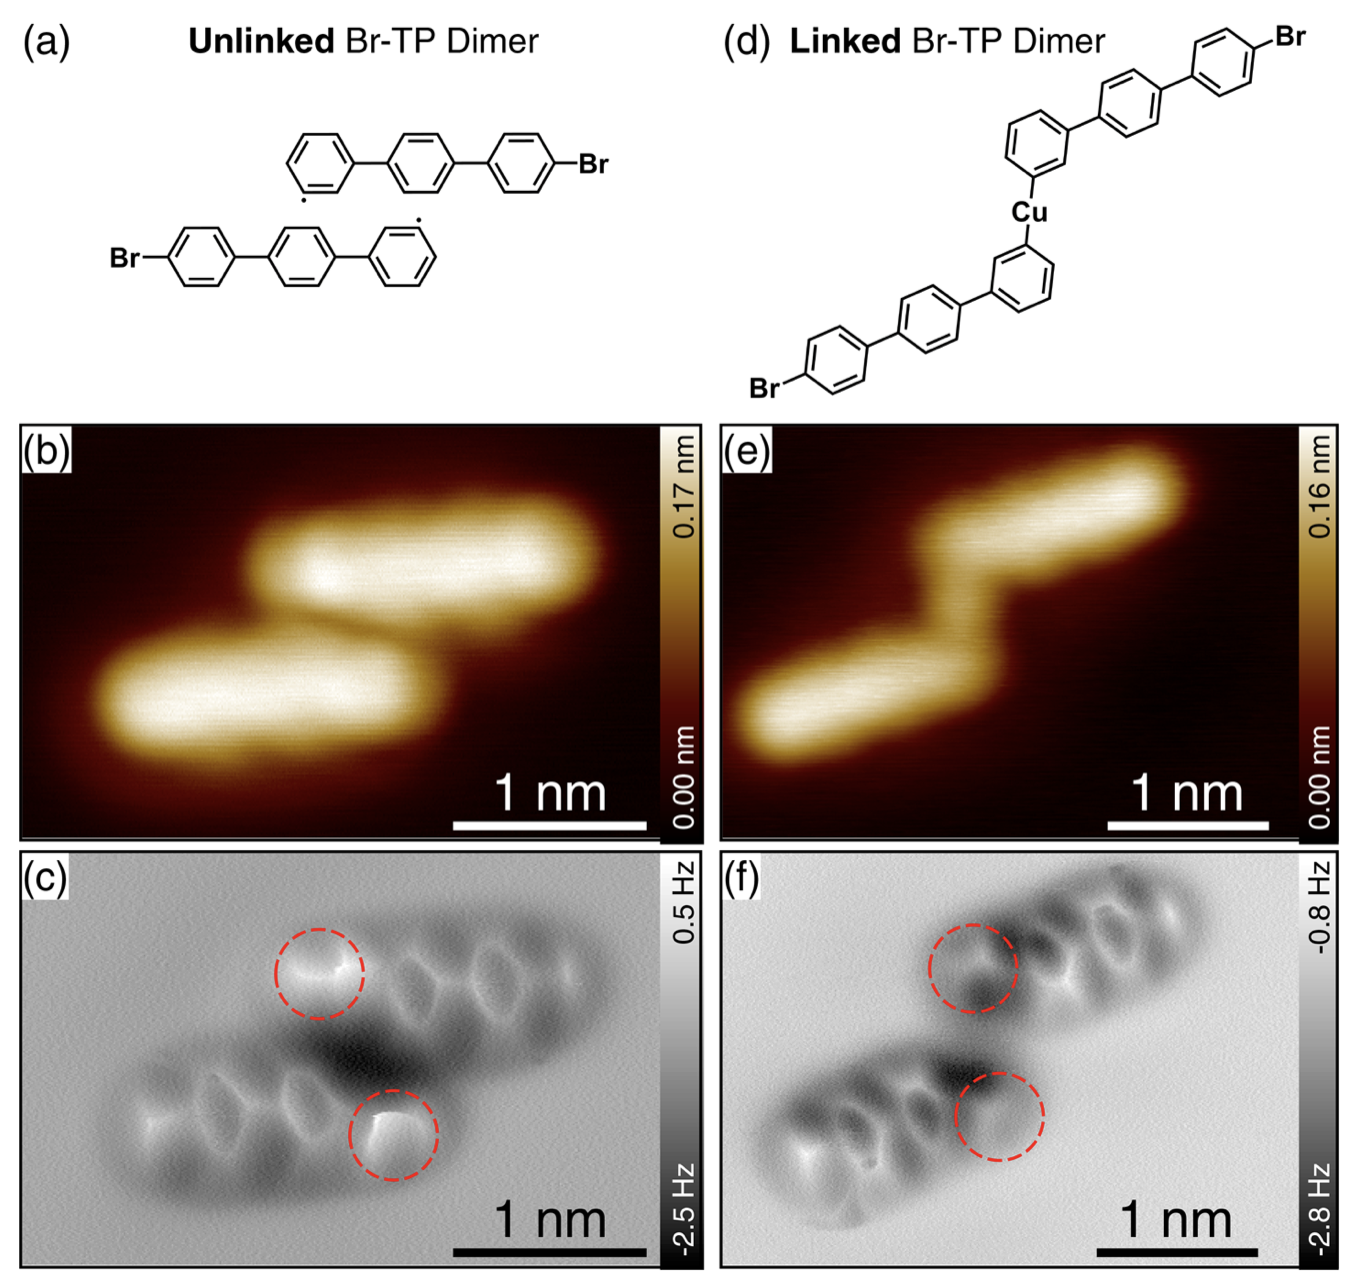
\includegraphics[width=0.98\columnwidth]{Fig/AFM_prove.png}
\caption{AFM}
\label{fig:6}
\end{figure}

In addition, chlorinated prophyrin as precursor has been deposited on Cu(111)~\cite{chematerial2019}. Based on DFT calculations, the Cu adatom mediated path is 3~eV lower than the direct dechlorination. And from STM image, some precursors are still intact at T 400~K, which should be already dehalogenated at lower T. It proves that the Cu adatoms are the limiting agent [Figure.~\ref{fig:prophyrin}].

\begin{figure*}[ht]
\centering
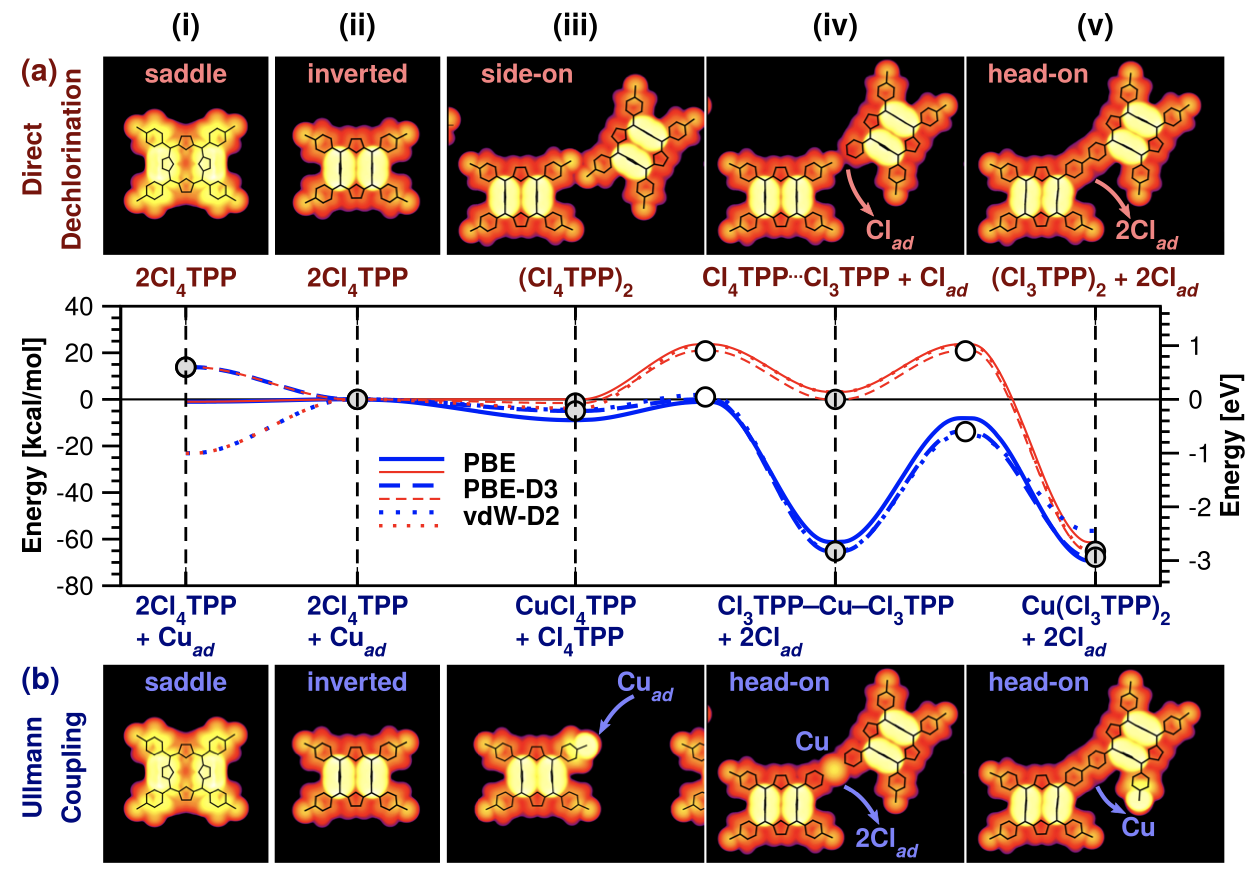
\includegraphics[width=0.98\textwidth]{Fig/Complete.png}
\caption{Prophyrin}
\label{fig:prophyrin}
\end{figure*}



\section{Methods}
\subsection{Computation Models}

The simulation of surface Ullmann coupling reaction was conducting with chlorobenzene, bromobenzene and iodobenzene on Cu(111) surface. We explored the four parts discussed above step by step. 

\subsection{Computational Details}

Density functional theory calculations were performed using the Perdew–Burke-Ernzerhof (PBE) for the exchange-correlation functional, the projector augmented wave method and a plane-wave basis set as implemented in the Vienna ab-initio simulation package . The energy cut-off for the plane-wave basis was set to 800 eV and a $3\times 3 \times1$ k-mesh was adopted. The mesh density of k points was kept fixed when performing related calculations with primitive cells. In optimizing the system geometry, van der Waals (vdW) interactions were considered by the DFT-D3 method. For the calculation of chlorobenzene, bromobenzene and iodobenzene adsorption on the Cu(111) surface, a slab consists of 192 Cu atoms arranging in 4 layers (a $48\times 4$ supercell was used), and the molecule was put on the center of the slab. Calculations were performed with applying spin-polarization. All atoms were fully relaxed until the MAX force on the atom was less than $2x10^{-2} eV/\si{\angstrom}^{2}$. 
For the Climbing-Image Nudged Elastic Band methods (CI-NEB) calculations, Using an improved initial guess~\cite{ullmann_60} instead of linear interpolation for minimum energy path in CI-NEB calculation, different number of intermediates were interpolated between the initial and final configurations due to the distance between them. Plus, All atoms were fully relaxed until the MAX force on the atom was less than $0.1 eV/\si{\angstrom}^{2}$ in CI-NEB calculations.



\section{Results and Discussion}



\subsection{Dehalogenation}

The dehalogenation is the common initialization of surface Ullmann coupling, to study this step and how different halogens would affect the dehalogenation reaction, We applied CI-NEB into three molecular precursors: chlorobenzene, bromobenzene and iodobenzene on the same Cu(111) surface after geometry optimizations. CI-NEB method offered us reaction coordinate diagram as well the transition state.

(In the literature, they mentioned that in the gas phase, the dissociation reaction are highly endothermic (3.85 eV for bromobenzene and 3.33 eV for iodobenzene), we can get the energy for this reaction too)

Figure.~\ref{fig:dissociation_Cl}, Figure.~\ref{fig:dissociation_Br} and Figure.~\ref{fig:dissociation_I} shows the initial, transition and final states (notated as IS, TS and FS, respectively) of chlorobenzene, bromobenzene and iodobenzene dihalogenation on Cu(111), respectively. 

Firstly, these three reactions are all exothermic, which turned out to be endothermic in gas phase. This is due the formation of energetically unstable radical in gas phase, but copper surface can donate electrons to stable these intermediate species. The enthalpy ($\Delta H$ = $E_{FS} - E_{IS}$) of dehalogenation of chlorobenzene, bromobenzene and iodobenzene on Cu(111) are -0.58 eV, -0.8 eV and -0.94 eV, respectively. In the FS figure, the halogens always sitted on the hollow site of Cu(111) surface. In IS, the precursor molecule was physisorbed by the surface, the adsorption energy are 1.06 eV, 1.18 eV and 1.37 eV, respectively for chlorobenzene, bromobenzene and iodobenzene. In TS, the geometry of chlorobenzene, bromobenzene and iodobenzene on Cu(111) are similar, forming a tilt angle, ready for the break of carbon-halogen bonds (C-X), the distance of C-X are 2.18 \si{\angstrom}, 2.46 \si{\angstrom} and 2.61 \si{\angstrom}, respectively. After dehalogenation, the phenyl species and halogen atom were separately chemisorbed by Cu(111) surface. In FS, the distance between the carbon (form C-X bond in IS) and halogen are 3.99 \si{\angstrom}, 4.10 \si{\angstrom} and 5.10 \si{\angstrom}, respectively. The geometry of TS for chlorobenzene, bromobenzene are similar, which displayed a more tilt angle compared to the TS. However. In the TS of iodobenzene, the phenyl specie is almost vertical to the copper surface. This makes a contribution to the highest enthalpy of iodobenzene dehalogenation. Another reason why iodobenzene possesses the highest enthalpy may come from the strongest chemisorption of Iodine on Copper. 

Secondly, the rate of a reaction would depend on $E_{barrier}$ rather than the enthalpy. Here we summarized the $E_{barrier}$ ($E_{barrier} = E_{TS} - E_{IS}$) for three halogenation reaction, which are 1.25 eV, 0.92 eV and 0.68 eV, respectively. These $E_{barrier}$ values indicate that the carbon-iodine bond is the easiest to break on Cu(111) surface while the carbon-chlorine bond is the hardest. This is consistent with the experimental data that in room temperature, most carbon-iodine and carbon-bromine bonds will dissociate while an higher temperature is required to break all carbon-chlorine bond in surface Ullmann coupling.

Summarizing the dehalogenation results, the reaction mechanism of chlorobenzene, bromobenzene and iodobenzene are very comparable on Cu(111) surface, the geometry of TS are analogous. The phenyl species of chlorobenzene, bromobenzene form a tilt angle with copper surface and it is vertical in iodobenzene case. The dehalogenation of iodobenzene is the easiest among these three reactions due to the lowest activation energy.


\begin{figure*}[ht]
\centering
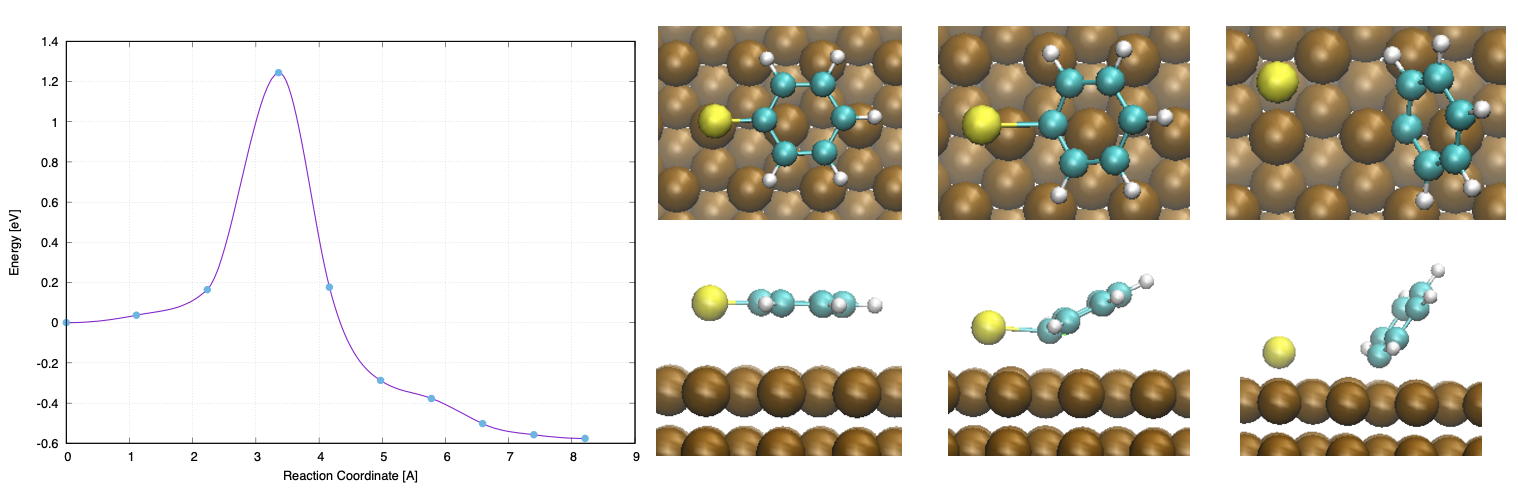
\includegraphics[width=0.98\textwidth]{Fig/dissociation_Cl.png}
\caption{The dissociation of C-Cl bond on Cu(111) surface, left is the energy diagram of the CI-NEB calculations, right side are the top and side view of $IS$, $TS$ and $FS$. (Sphere with ochre color is copper atoms, with cyan color is carbon atoms, with white color is hydrogen atoms. Same in below models. Sphere with yellow color is chlorine atom)}
\label{fig:dissociation_Cl}
\end{figure*}

\begin{figure*}[ht]
\centering
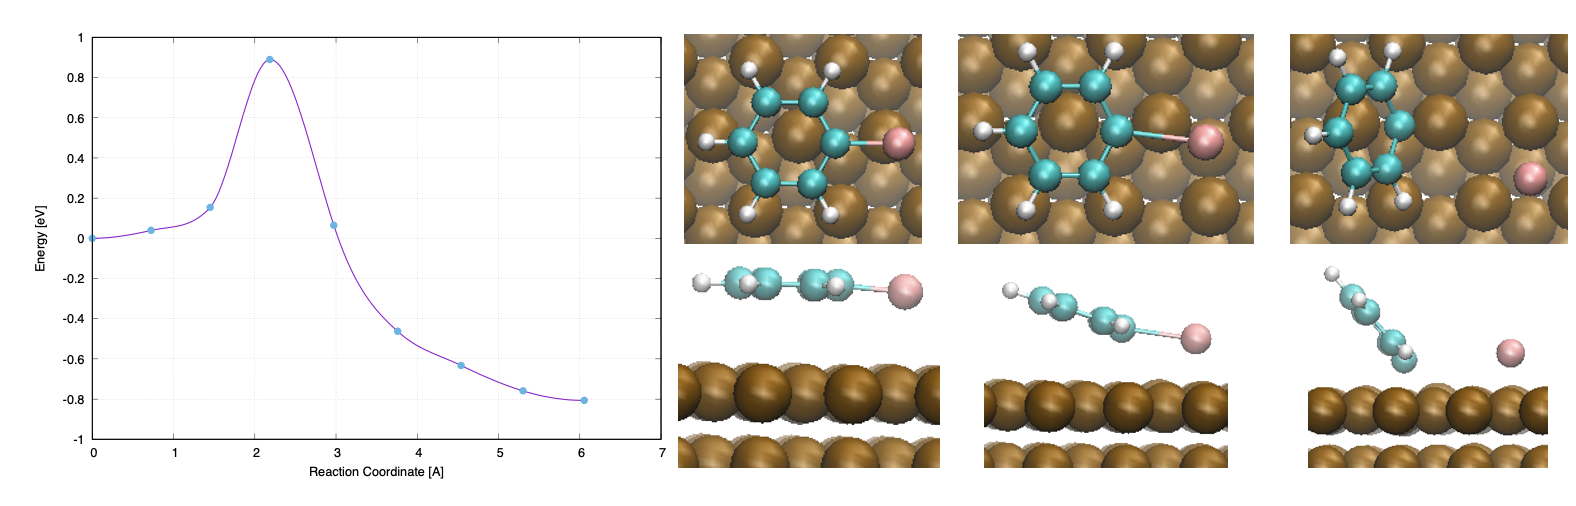
\includegraphics[width=0.98\textwidth]{Fig/dissociation_Br.png}
\caption{The dissociation of C-Br bond on Cu(111) surface. (Sphere with lime color is bromine atoms)}
\label{fig:dissociation_Br}
\end{figure*}

\begin{figure*}[ht]
\centering
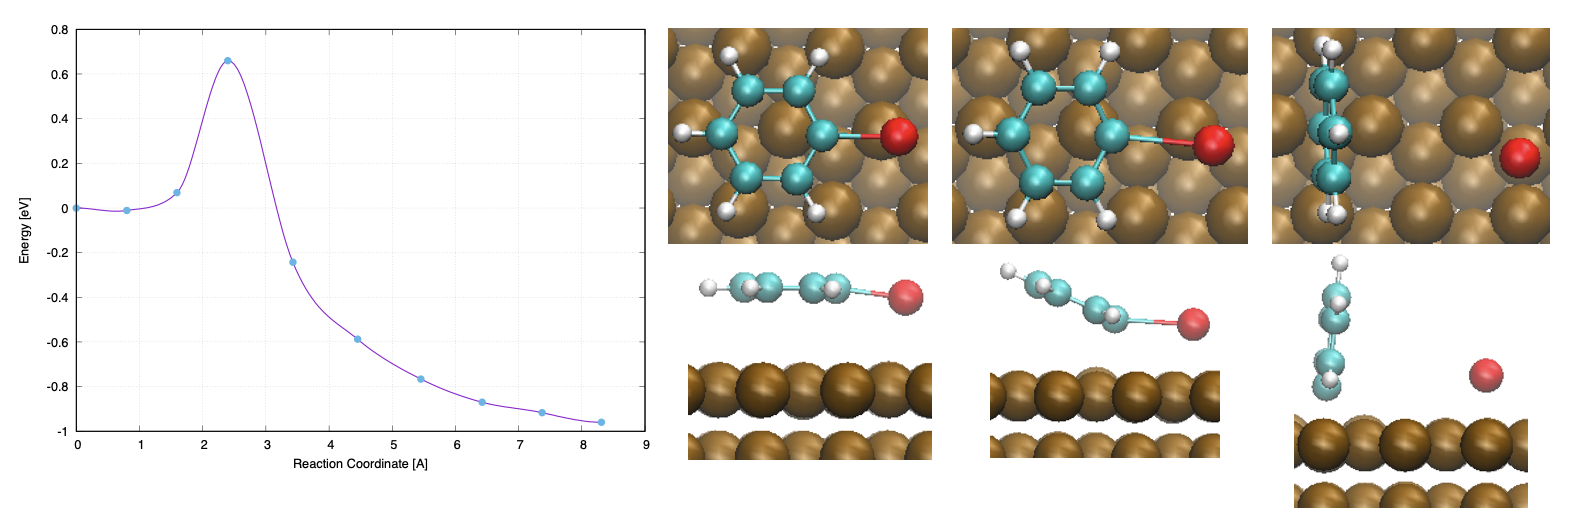
\includegraphics[width=0.98\textwidth]{Fig/dissociation_I.png}
\caption{The dissociation of C-I bond on Cu(111) surface. (Sphere with red color is iodine atoms)}
\label{fig:dissociation_I}
\end{figure*}


\subsection{Diffusion and Formation of Dimerized Organometallic Intermediates}

After the dehalogenation, the diffusion of all species on copper surface would possibly bring two orientation-matched phenyl groups together, leading to the formation of dimerized organometallic intermediates. Since the halogens such as chlorine, bromine and iodine have been chemisorbed by the surface, the organometallic intermediate could be fairly considered as the same state for all three precursors to reach.

Figure.~\ref{fig:organometallicintermediate} shows the optimized geometry of organometallic intermediate on Cu(111) surface. From the left picture, it is apparent that these two phenyl groups both conducted interactions with the copper atom on Cu(111) surface; from the right side, it shows that, the copper atom that interacted with two phenyl groups is partially lifted from the first layer flat. And this phenomenon does not appear when there is only one phenyl group. 
Besides, the enthalpy of the reaction for three precursors from dehalogenated chlorobenzene, bromobenzene and iodobenzene to dimerized organometallic intermediate are +1.40 eV, +0.17 eV and +0.17 eV, respectively. These three reactions are all endothermic, and the dehalogenated chlorobenzene will adsorb the most heat, which is consistent with the experiment that transformation to organometallic intermediates of dichlorobenzenes wound not be completed unless a higher temperature is present, but transformation of dibromobenzenes and diiodobenzenes would fulfill at room temperature.

Here, we considered that the organometallic intermediates were formed with the copper atom which is original located in the surface. In reality, the copper atom in organometallic intermediates may also come from the adatom which already lay on the surface before the coupling reaction. In this case -----

\begin{figure*}[ht]
\centering
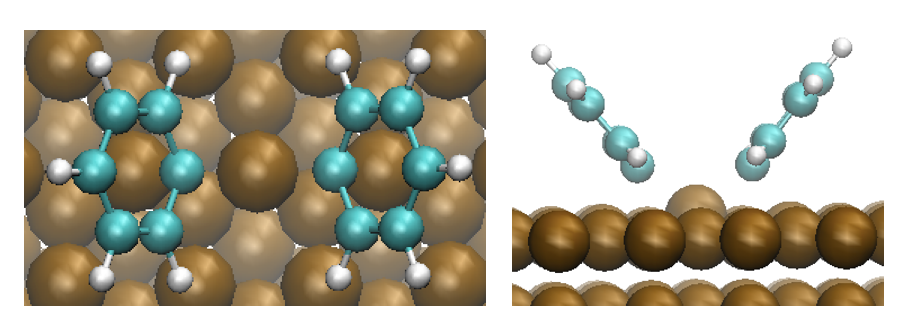
\includegraphics[width=0.98\textwidth]{Fig/organometallicintermediate.png}
\caption{The organometallic intermediate on Cu(111) surface}
\label{fig:organometallicintermediate}
\end{figure*}

\subsection{Formation of Carbon Carbon (C-C) Bond}

The final coupling step is the formation of carbon carbon bond (C-C). As discussed above, we explored the two pathways of the formation: (1) the Cu atom is partially lifted from the surface and back in the surface after the formation of C-C bond; (2) the Cu atom is partially lifted from the surface and then fully pulled out to become an adatom on top of the surface then take part in the formation.
Here we investigated two possibilities separately.

\subsubsection{Path I: Cu Returns to Original Location after Coupling Reaction}

In Path I, the formation started from the organometallic intermediate in which the copper atom was partially lifted (notated as $IS_{path1}$). Then the two carbons which would construct a new bond later slope closer to each other, while the copper atom was less lifted on the surface (notated as $TS_{path1}$). Finally, a new C-C bond was formed and the surface went back to original geometry without vacancy (notated as $FS_{path1}$).

In Figure.~\ref{fig:bondformlift}, along the potential energy surface, 6 intermediates were interpolated between $IS_{path1}$ and $FS_{path1}$. The tilt angle of phenyl species in respect to the Cu(111) surface initialized at $50^\circ$ in $IS_{path1}$, then flattened to $35^\circ$ in $TS_{path1}$ and ended at $0^\circ$ in $FS_{path1}$. The distance between the two carbons which would construct a bond varied from 3.10 \si{\angstrom} to 2.28 \si{\angstrom} and ended at 1.49 \si{\angstrom}.

Path I reaction is exothermic, the enthalpy $\Delta H$ is $-2.00 eV$, and $E_{barrier}$ is $0.50 eV$.

\begin{figure*}[ht]
\centering
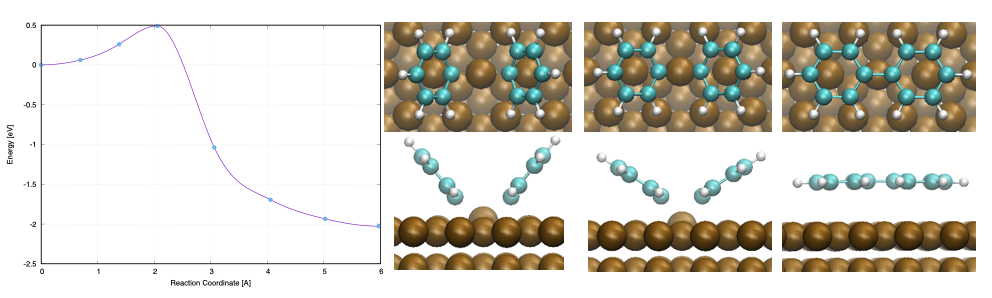
\includegraphics[width=0.98\textwidth]{Fig/bondformlift.png}
\caption{C-C bond formation through lifting Cu atom Path I}
\label{fig:bondformlift}
\end{figure*}


\subsubsection{Path II: Cu becomes a new adatom after coupling reaction}

In Path II, the process started from the organometallic intermediate whereh the copper atom is fully pulled out as an adatom (notated as $IS_{path2}$) (here we created a vacancy on surface corresponding to the creation of adatom, to assure the whole system has the same number of atoms). Then the two phenyl groups would be lifted higher and closer to each other, while the copper atom is less lifted and move towards a hollow site on the surface(notated as $TS_{path2}$). Finally, a new C-C bond is formed and a new adatom and a new vacancy are created on the surface (notated as $FS_{path2}$).

As Figure.~\ref{fig:bondformadatom} show, in this path, 10 intermediates were interpolated between $IS_{path2}$ and $FS_{path2}$.The tilt angle of phenyl species in respect to the Cu(111) surface initialized at $8.5^\circ$ and $12.2^\circ$ in $IS_{path2}$ (the difference angle could be accounted by the fact that vacancy is close the one phenyl species, this will affect a little on the tilt angle), then flattened to nearly $0^\circ$ in $TS_{path2}$ and ended at $-9.1^\circ$ in $FS_{path2}$ (the negative angle arises from the fact that the adatom is right behind the biphenyl). The distance between the two carbons which would construct a bond varied from 3.89 \si{\angstrom} to 2.53 \si{\angstrom} and ended at 1.50 \si{\angstrom}.

Path II reaction is slightly exothermic, the enthalpy $\Delta H$ is $-0.17 eV$, and $E_{barrier}$ is $2.00 eV$, higher than the $E_{barrier}$ of Path I.

\begin{figure*}[ht]
\centering
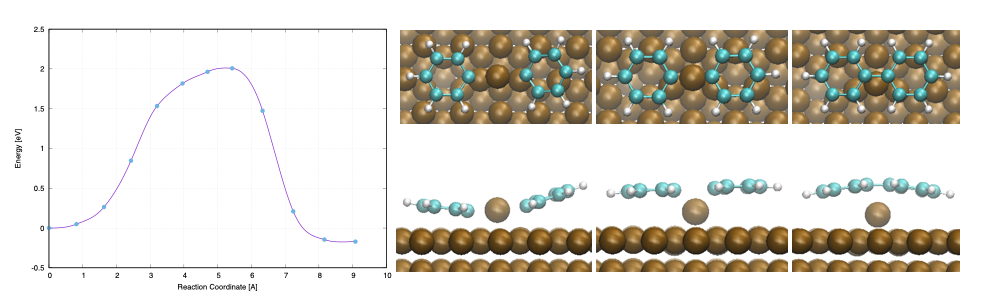
\includegraphics[width=0.98\textwidth]{Fig/bondformadatom.png}
\caption{C-C bond formation through new formed adatom Path II}
\label{fig:bondformadatom}
\end{figure*}

\subsubsection{Path I Vs Path II}

Taking the data of Path I and Path II both into consideration, finally, a plausible C-C bond was constructed in both case (bond length is around $1.5$ \si{\angstrom}, expected to be 1.34 \si{\angstrom} - 1.54 \si{\angstrom}) From thermodynamic aspect, Path I is much more exothermic, which means it will lead to a more stable product. Kinetically, the activation energy of Path I is also smaller than Path II, which means at the same temperature, the Path I reaction would take place at a higher speed and account for a much larger probability in reality. In this case, we could safely conclude that, if there is no pre-exiting adatom on copper surface, the formation of C-C bond in surface Ullmann coupling will follow the path I.\\

\subsection{Energy Diagram of Complete Surface Ullmann Coupling Reaction}
In this section, the summary of thermodynamic data of all intermediates in surface Ullmann coupling reaction is present in one diagram. As is shown in Figure.~\ref{fig:completeenergy}.
Here taking the surface Ullmann coupling between two bromobenzene obtaining biphenyl as example,
The physisorption of two bromobenzene on Cu(111) surface decrease the energy of the whole system by 2.35 eV, which is widely recognized in experiment that it is a fast process for copper surface to adsorb aromatic species. 
And then till the formation of new C-C bond, a detailed discussion has been demonstrated in previous sections. The last two successive steps are concerned with the desorption of biphenyl molecule and two dehalogenated bromine atoms. 
In total, the red line is more energetically favourable than green line, that might considered to be a more reasonable pathway in reality surface Ullmann coupling if there is no pre-exiting adatom on metal surface.

\begin{figure*}[ht]
\centering
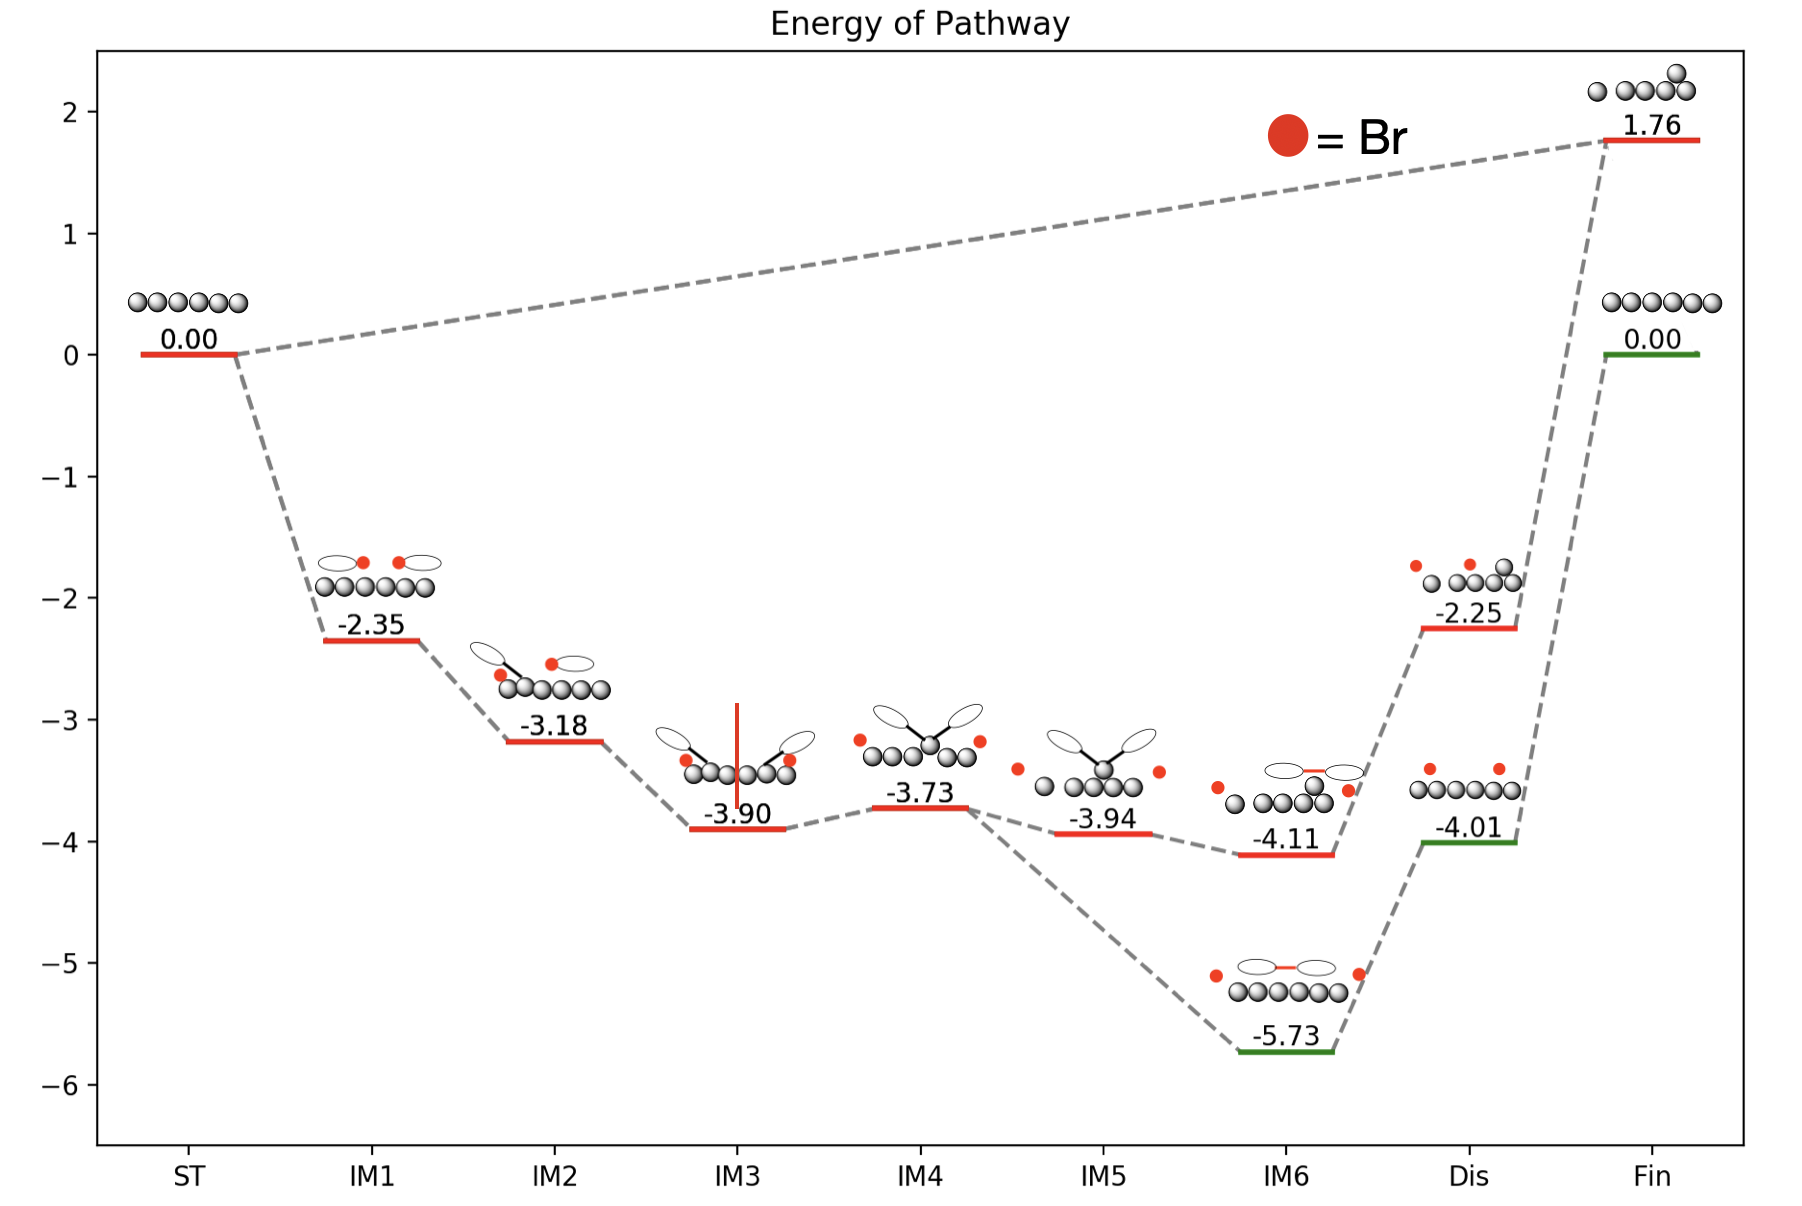
\includegraphics[width=0.72\textwidth]{Fig/completeenergy.png}
\caption{The Energy Diagram of Surface Ullmann Coupling Reaction.
the red line is the surface Ullmann Coupling reaction following Path II, the green line is following Path I. Finally, red line ended with a adatom-vacancy pair on Cu(111) surface and the green line ended same as the original Cu(111) surface.(red circle means bromine atoms)}
\label{fig:completeenergy}
\end{figure*}

\subsection{Formation of Adatom on Pure Cu Surface}

Finally, the energy of forming adatom on a pure Cu surface is also present. The goal of obtaining this energy diagram is to launch a comparison between two different conditions to deliver a adatom on Cu(111) surface. 
As Figure.~\ref{fig:pureadatomform} shows, the reaction of forming a new adatom-vacancy pair on pure Cu(111) surface is endothermic, $\Delta H$ is 1.76 eV and the $E_{barrier}$ is 2 eV. This means at room temperature, the formation of adatom is unfavourable. 
However, as is shown in Figure.~\ref{fig:completeenergy}, the presence of organometallic intermediate in surface Ullmann coupling could promote the formation of adatoms on surface both thermodynamically and kinetically. This pathway might be considered as a plausible method to create adatom on metal surface.

\begin{figure*}[ht]
\centering
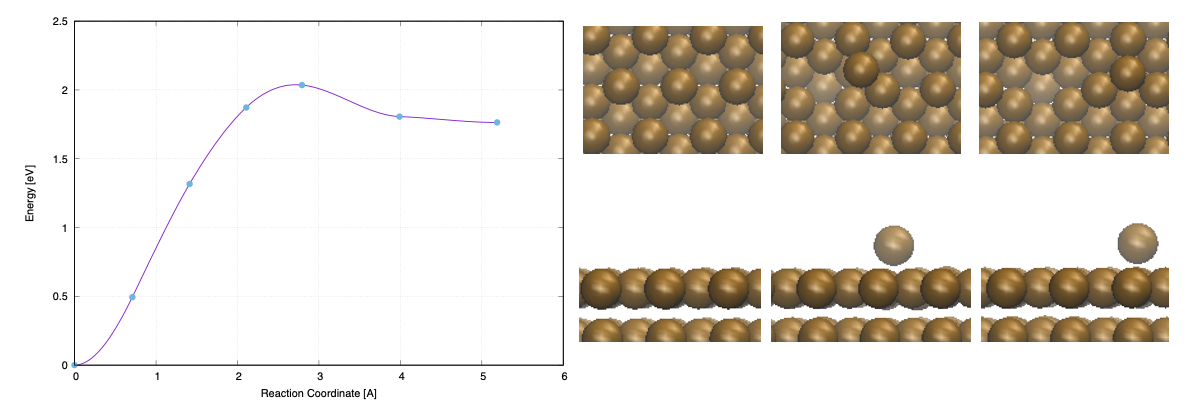
\includegraphics[width=0.98\textwidth]{Fig/pureadatomform.png}
\caption{adatom formation on pure Cu(111) surface}
\label{fig:pureadatomform}
\end{figure*}



\bibliographystyle{unsrt}  
\bibliography{references.bib}  %%% Remove comment to use the external .bib file (using bibtex).
%%% and comment out the ``thebibliography'' section.




\end{document}
